\appendix

\section{Results from ASA}
\label{apx:tools}

\begin{figure}[h!]
	\centering
	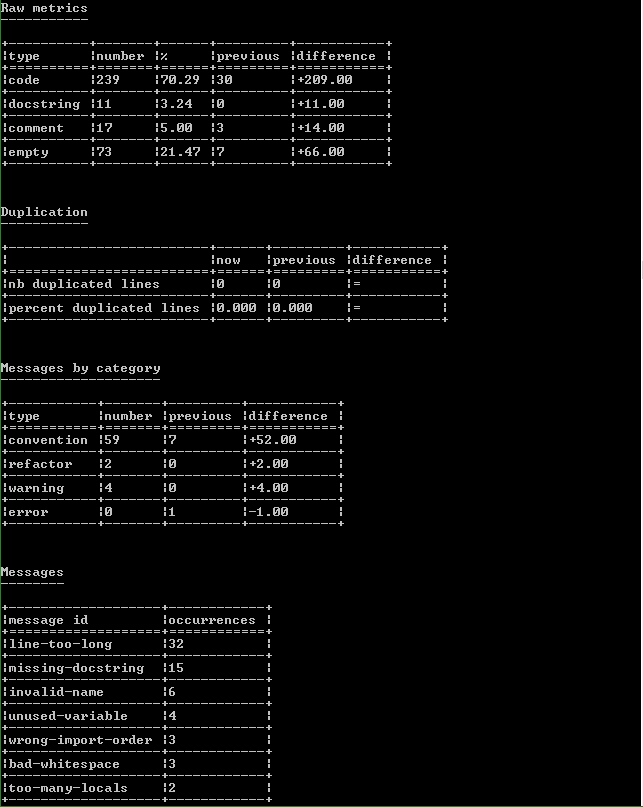
\includegraphics[width=.8\textwidth, keepaspectratio]{graphics/pylint_tools_3}
	\caption{Pylint messages for \texttt{evaluation/tools.py}}
\end{figure}

\begin{figure}[h!]
	\centering
	
\includegraphics[width=.8\textwidth, keepaspectratio]{graphics/pylint_tools_4}
	\caption{Pylint rating for \texttt{evaluation/tools.py}}
\end{figure}

\begin{figure}[h!]
	\centering
	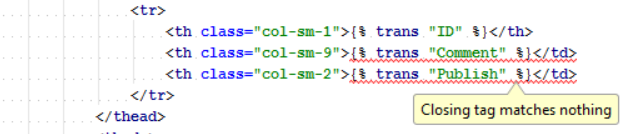
\includegraphics[width=.8\textwidth, keepaspectratio]{graphics/pyCharmInspection-closingTagMatchesNothing}
	\caption{PyCharm Inspection result: the closing tag must be a \texttt{</th>} as well.}
\end{figure}

\begin{figure}[h!]
	\centering
	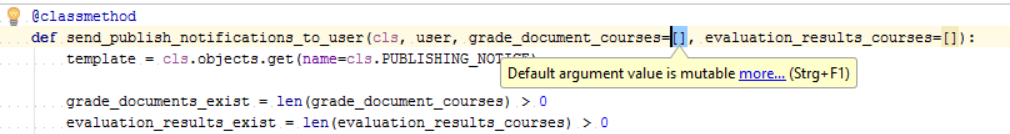
\includegraphics[width=.8\textwidth, keepaspectratio]{graphics/pyCharmInspection-defaultArgumentValueIsMutable}
	\caption{PyCharm's Inspection finds the same dangerous default argument as Landscape.}
\end{figure}

\begin{figure}[h!]
	\centering
	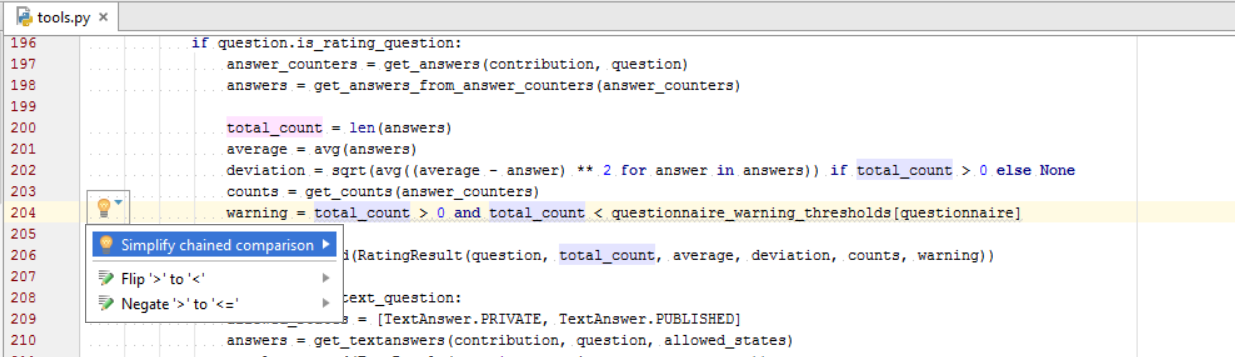
\includegraphics[width=.8\textwidth, keepaspectratio]{graphics/pyCharmInspection-simplifyChainedComparison}
	\caption{PyCharm suggests code changes for better code style.}
\end{figure}

\begin{figure}[h!]
	\centering
	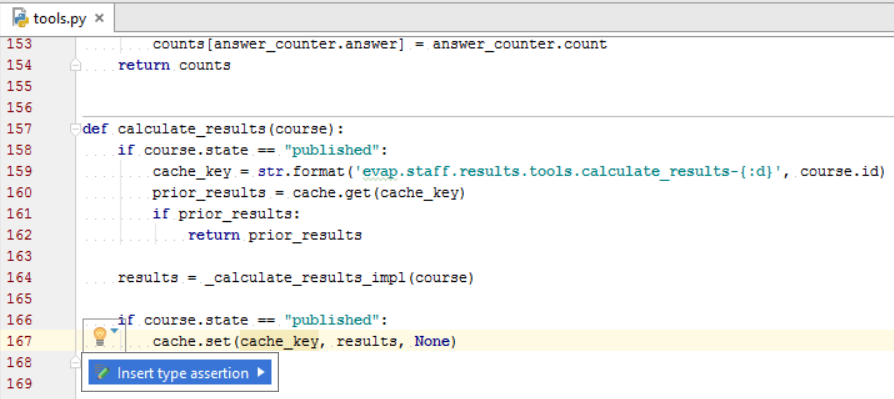
\includegraphics[width=.8\textwidth, keepaspectratio]{graphics/pyCharmInspection-unboundLocalVariable}
	\caption{PyCharm cannot know that the course state does not change within the method and therefore believes, that the highlighted variable could be uninitialized.}
	\label{pic:pycharm-uninitialized}
\end{figure}
